\documentclass[10pt,conference,compsocconf]{IEEEtran}

\usepackage[T1]{fontenc}
\usepackage{hyperref}
\usepackage{graphicx}
\usepackage{booktabs}
\usepackage{amsmath}
\usepackage{amssymb}

\begin{document}
\title{Predicting Coronary Heart Disease\\from the 2015 BRFSS Survey}

\author{
  Tommaso Sommaruga, Paolo Ferrari, Francesco Foglia\\
  \textit{CS-433 Machine Learning, Project 1, EPFL, Switzerland}
}

\maketitle

\begin{abstract}
We predict from the 2015 Behavioral Risk Factor Surveillance System (BRFSS)
whether a respondent reports coronary heart disease or a heart attack (MICHD);
only 8.8\% of the 328{,}135 training rows are positive, so we optimise the
positive-class F1. On the same features as the six course methods, a small
neural network (Linear--BatchNorm--ReLU) fits the training data better but does
not beat logistic regression on held-out data (F1 0.425 versus 0.429): the limit
is the signal in the features, not the model capacity. The gains come from the
preprocessing: treating every answer code as a category and keeping the 300
one-hot levels with the highest mutual information beats other encodings by up
to 0.08 F1. Our class-weighted logistic regression reaches a 5-fold F1 of
$0.427\pm0.002$ and an AIcrowd F1 of 0.439 (accuracy 0.877).
\end{abstract}

\section{Introduction}
Cardiovascular diseases are a leading cause of death. The BRFSS telephone survey of the U.S.
Centers for Disease Control and Prevention records health status, chronic
conditions and lifestyle of U.S.\ adults. From the 321 answers of a respondent
we predict the label $y\in\{-1,+1\}$ (MICHD). We compare the six methods seen in
class with a small neural network, to test whether more capacity helps; since it
does not, we focus on the preprocessing.
Only NumPy and Matplotlib are used; \texttt{run.py} reproduces our best AIcrowd
submission.

\section{Models and Methods}
\subsection{Data and exploratory analysis}
The training set has 328{,}135 rows and the test set 109{,}379, both with 321
features. 44.8\% of the cells are blank in both sets, 147 columns are more than
half empty (optional modules, skip patterns) and 6 are constant.
Most columns are coded categories: on day-count questions 88 means ``none'' and
77/99 mean ``don't know''/``refused'', so the numeric value is meaningless.
The positive rate grows from 0.5\% at age 18--24 to 22.2\% at 80+, and is
11.2\% for men versus 7.1\% for women. On 87 columns the missing rate differs
between the classes by more than 5 points, so a blank is itself informative.
Four items on cardiac and stroke rehabilitation and aspirin use
(\texttt{HAREHAB1}, \texttt{STREHAB1}, \texttt{CVDASPRN}, \texttt{ASPUNSAF}) concern only
people with a cardiac history; we treat them as label leaks.

\subsection{Preprocessing}
The pipeline of \texttt{src/preprocessing.py} is fitted on training rows only,
then frozen and applied to validation and test rows.
\begin{enumerate}
\item \emph{Column removal.} We drop 40 columns that describe the interview
rather than the person (state, dates, sequence number, phone checks, sampling
weights), the 4 leak columns, and columns that are empty or constant.
\item \emph{Level encoding.} Each remaining column becomes indicator (one-hot)
levels. A value held by at least 1\% of the rows gets its own level, so special
codes such as 77, 88 and 99 stay separate categories; the rarer values are cut
into at most 5 quantile bins (or pooled into one level), and ``missing'' is a
level when at least 1\% of the rows are blank.
\item \emph{Selection.} Constant and duplicate indicators are removed (about
1{,}750 remain) and the 300 with the highest mutual information with the label
are kept. They come from 143 raw columns.
\item \emph{Standardisation} with the training mean and standard deviation.
\end{enumerate}

\subsection{Course methods}
We compare the six required methods: least squares with gradient descent (GD)
and with stochastic gradient descent (SGD, batch size 1), least squares and
ridge regression with the normal equations, and logistic and
$\ell_2$-regularised logistic regression with GD (all in
\texttt{implementations.py}).
We fit them on the preprocessed matrix plus a bias column, with targets
$y\in\{0,1\}$, zero initialisation and the grids of Table~\ref{tab:methods}.
GD step sizes are fractions of the stability limit, $2/L$ for the squared and
$8/L$ for the logistic loss, where $L=29.7$ is the top eigenvalue of $X^{\top}X/n$.

\subsection{Neural network}
We implemented in NumPy (\texttt{neural\_net.py}) a multilayer perceptron with two
hidden layers of 128 and 64 units, each Linear $\to$ BatchNorm $\to$ ReLU, and a
linear output (He initialisation). \texttt{train.py} trains it on the same
features with binary cross-entropy, positives weighted by
$n_{-}/n_{+}=10.3$, Adam (learning rate $\in\{10^{-3},10^{-4}\}$, weight decay
$\in\{0,0.1\}$), batches of 256 and early stopping on the tune-slice loss
(patience 5).

\subsection{Submitted model}
Let $y_i\in\{0,1\}$ and give each row a weight $w_i$ such that the positive rows
together weigh twice the negative ones. We minimise
\begin{equation}
\min_{\theta}\;\frac{1}{n}\sum_{i=1}^{n} w_i\,
\ell\!\left(y_i,\theta_0+x_i^{\top}\theta_{1:}\right)
+\lambda\|\theta_{1:}\|_2^2 ,
\label{eq:obj}
\end{equation}
with $\ell(y,s)=\log(1+e^{s})-ys$ and $\lambda=10^{-5}$ (the bias is not
penalised), by 300 steps of FISTA (Nesterov-accelerated gradient descent) with step
$1/(1.1\,\hat L/4+2\lambda)$, $\hat L$ being the top eigenvalue of the weighted Gram matrix.

\subsection{Decision threshold and validation}
For a rare class F1 is not maximised at probability 0.5. Inside every training
set we hold out a stratified 15\% \emph{tune} slice and choose the score cut $t$
that maximises F1 among 201 quantiles of the tune scores.
The generalisation error is estimated by stratified 5-fold cross-validation
(seed 42): in each fold, preprocessing and model are fitted on 85\% of the four
training folds, $t$ on the other 15\%, and the held-out fold is scored once.
For Table~\ref{tab:methods} we use fold~0 (65{,}627 held-out rows) and also pick
each method's hyperparameters on the tune slice.
The submission (\texttt{run.py}, settings in
\texttt{config/experiments.json}) repeats the 85/15 procedure on all labelled
rows; it gives $t=1.75$, labels 13.16\% of the test rows positive and writes
\texttt{submissions/weighted\_logistic.csv}.

\section{Results}
\begin{table}[t]
\centering
\caption{All models on fold 0: F1 of the positive class (MICHD) on the
held-out rows (same features and protocol; setting chosen by F1 on the tune
slice).}
\label{tab:methods}
\footnotesize
\setlength{\tabcolsep}{4pt}
\begin{tabular}{llcc}
\toprule
Method & Setting & F1 & PR-AUC \\
\midrule
Least squares (normal eq.) & -- & 0.419 & 0.386 \\
Ridge regression & $\lambda=10^{-2}$ & 0.421 & 0.385 \\
Least squares, GD & $\gamma=0.034$ & 0.420 & 0.385 \\
Least squares, SGD & $\gamma=10^{-4}$ & 0.413 & 0.371 \\
Logistic regression, GD & $\gamma=0.13$ & 0.429 & \textbf{0.396} \\
Reg.\ logistic regression, GD & $\lambda=10^{-3}$, $\gamma=0.13$ & \textbf{0.430} & \textbf{0.396} \\
\midrule
MLP 128--64, BN, ReLU & lr $=10^{-3}$, wd $=0$ & 0.425 & 0.385 \\
Weighted logistic, FISTA$^{\ast}$ & $\lambda=10^{-5}$ & 0.427 & 0.392 \\
\bottomrule
\multicolumn{4}{p{0.95\columnwidth}}{\raggedright\scriptsize Grids: ridge
$\lambda\in\{10^{-5},\dots,10^{-2}\}$; GD $\gamma\in\{0.017,0.034,0.064\}$;
SGD $\gamma\in\{10^{-4},10^{-3}\}$ ($2\cdot10^{5}$ steps); logistic
$\gamma\in\{0.067,0.13,0.26\}$; reg.\ logistic
$\lambda\in\{10^{-4},10^{-3},10^{-2}\}$; GD methods 500 steps.
$^{\ast}$Submitted.} \\
\end{tabular}
\end{table}

\begin{table}[t]
\centering
\caption{Preprocessing ablation with the submitted model: 5-fold means
(standard deviation of F1 between 0.001 and 0.003).}
\label{tab:ablation}
\footnotesize
\setlength{\tabcolsep}{4pt}
\begin{tabular}{lcccc}
\toprule
Representation & F1 & PR-AUC & ROC-AUC & Cols \\
\midrule
One-hot, MI top 300$^{\ast}$ & \textbf{0.427} & \textbf{0.388} & \textbf{0.861} & 300 \\
One-hot, all levels, $\ell_1$ & 0.425 & 0.385 & 0.859 & 1753 \\
One-hot, all levels & 0.422 & 0.382 & 0.857 & 1753 \\
Codebook recode & 0.422 & 0.386 & 0.859 & 171 \\
Codebook + one-hot & 0.422 & 0.382 & 0.857 & 1924 \\
One-hot $\times$ (age $\ge$ 65) & 0.422 & 0.381 & 0.857 & 1864 \\
Numeric, median + flags & 0.410 & 0.359 & 0.851 & 464 \\
Same, $<$50\% missing cols & 0.407 & 0.355 & 0.850 & 215 \\
Numeric + flags on top 40 & 0.395 & 0.336 & 0.841 & 227 \\
Missing flags only & 0.343 & 0.270 & 0.807 & 187 \\
\bottomrule
\multicolumn{5}{l}{\scriptsize $^{\ast}$Submitted representation.} \\
\end{tabular}
\end{table}

\begin{figure}[t]
\centering
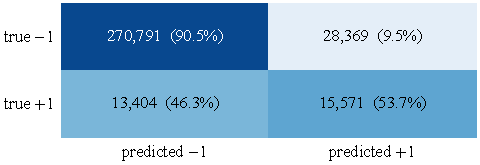
\includegraphics[width=0.92\columnwidth]{confusion_matrix.pdf}
\caption{Submitted model, pooled over the five held-out folds (row
percentages): precision 0.354, recall 0.537, F1 0.427, accuracy 0.873.}
\label{fig:cm}
\end{figure}

\emph{Course methods.} The six methods span 0.413--0.430 F1
(Table~\ref{tab:methods}); the logistic loss beats the squared loss by about
0.01 in F1 and PR-AUC.
SGD with batch size 1 is the weakest.

\emph{Neural network.} The setting chosen on the tune slice reaches F1 0.425
(others 0.424--0.426), no better than logistic regression (0.429). Its tune loss is
lowest after only 2 epochs and it fits its training rows better than it
generalises (F1 0.445 versus 0.425), while logistic regression shows no gap
(0.430 versus 0.429). The linear model is thus not underfitting, and extra
capacity only fits noise: the limit is the signal in the features. We submit the
weighted logistic regression (used for Table~\ref{tab:ablation}, best on AIcrowd).

\emph{Preprocessing ablation.} Table~\ref{tab:ablation} changes only the
representation (code: \texttt{src/pipeline\_experiments.py}, commit
\texttt{9c5b69a}). Reading the codes as numbers with median imputation and
missing flags loses 0.017 F1 and 0.029 PR-AUC. Missing flags alone lose 0.084
F1: blanks carry signal, but much less than the answers. A hand-made clinical
codebook, all 1{,}753 one-hot levels (with or without an $\ell_1$ penalty) or
products with an age $\ge 65$ flag reach at most 0.425: the extra columns
repeat what the 300 selected levels carry. On AIcrowd, better preprocessing raised
F1 from 0.391 to 0.439, close to the 5-fold estimate.

\section{Discussion}
Almost half of the positives (46.3\%) are scored like negatives
(Fig.~\ref{fig:cm}): this class overlap, not the model, bounds the score. With a tuned threshold the class weight barely matters (in earlier runs,
weights from 0.5 to 6 changed F1 by 0.001), but the threshold must match the metric: tuning
it for F2 drops F1 to about 0.38.

\section{Summary}
Baselines, a neural network and preprocessing ablations agree: the bottleneck
is the signal in the survey answers, so the gains came from the preprocessing
(5-fold F1 $0.427\pm0.002$, AIcrowd F1 0.439, accuracy 0.877).

\end{document}
